\section{Auswertung}
\label{sec:Auswertung}

% % Examples
% \begin{equation}
%   U(t) = a \sin(b t + c) + d
% \end{equation}
%
% \begin{align}
%   a &= \input{build/a.tex} \\
%   b &= \input{build/b.tex} \\
%   c &= \input{build/c.tex} \\
%   d &= \input{build/d.tex} .
% \end{align}
% Die Messdaten und das Ergebnis des Fits sind in Abbildung~\ref{fig:plot} geplottet.
%
% %Tabelle mit Messdaten
% \begin{table}
%   \centering
%   \caption{Messdaten.}
%   \label{tab:data}
%   \sisetup{parse-numbers=false}
%   \begin{tabular}{
% % format 1.3 bedeutet eine Stelle vorm Komma, 3 danach
%     S[table-format=1.3]
%     S[table-format=-1.2]
%     @{${}\pm{}$}
%     S[table-format=1.2]
%     @{\hspace*{3em}\hspace*{\tabcolsep}}
%     S[table-format=1.3]
%     S[table-format=-1.2]
%     @{${}\pm{}$}
%     S[table-format=1.2]
%   }
%     \toprule
%     {$t \:/\: \si{\milli\second}$} & \multicolumn{2}{c}{$U \:/\: \si{\kilo\volt}$\hspace*{3em}} &
%     {$t \:/\: \si{\milli\second}$} & \multicolumn{2}{c}{$U \:/\: \si{\kilo\volt}$} \\
%     \midrule
%     \input{build/table.tex}
%     \bottomrule
%   \end{tabular}
% \end{table}
%
% % Standard Plot
% \begin{figure}
%   \centering
%   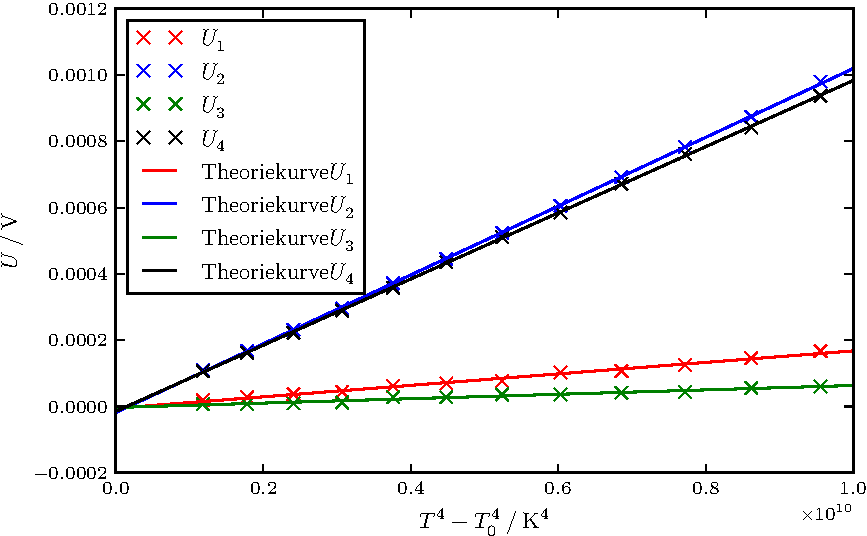
\includegraphics{build/plot.pdf}
%   \caption{Messdaten und Fitergebnis.}
%   \label{fig:plot}
% \end{figure}
%
% 2x2 Plot
% \begin{figure*}
%     \centering
%     \begin{subfigure}[b]{0.475\textwidth}
%         \centering
%         \includegraphics[width=\textwidth]{Abbildungen/Schaltung1.pdf}
%         \caption[]%
%         {{\small Schaltung 1.}}
%         \label{fig:Schaltung1}
%     \end{subfigure}
%     \hfill
%     \begin{subfigure}[b]{0.475\textwidth}
%         \centering
%         \includegraphics[width=\textwidth]{Abbildungen/Schaltung2.pdf}
%         \caption[]%
%         {{\small Schaltung 2.}}
%         \label{fig:Schaltung2}
%     \end{subfigure}
%     \vskip\baselineskip
%     \begin{subfigure}[b]{0.475\textwidth}
%         \centering
%         \includegraphics[width=\textwidth]{Abbildungen/Schaltung4.pdf}    % Zahlen vertauscht ... -.-
%         \caption[]%
%         {{\small Schaltung 3.}}
%         \label{fig:Schaltung3}
%     \end{subfigure}
%     \quad
%     \begin{subfigure}[b]{0.475\textwidth}
%         \centering
%         \includegraphics[width=\textwidth]{Abbildungen/Schaltung3.pdf}
%         \caption[]%
%         {{\small Schaltung 4.}}
%         \label{fig:Schaltung4}
%     \end{subfigure}
%     \caption[]
%     {Ersatzschaltbilder der verschiedenen Teilaufgaben.}
%     \label{fig:Schaltungen}
% \end{figure*}

\subsection{\texorpdfstring{Bestimmung von $\frac{h}{e_0}$ und der Austrittsarbeit}{Bestimmung von h/e und der Austrittsarbeit}.}

Um die Grenzspannungen zu bestimmen, wird für fünf Spektrallinien die Stromstärke in Abhängigkeit von der Gegenspannung gemessen.
Da das Verhältnis im Bereich der Grenzspannung als quadratisch angenommen werden kann, wird die Wurzel der Stromstärke jeweils gegen die Gegenspannung aufgetragen.
Mit diesen Werten wird jeweils ein linearer Fit mit SciPy in Python erstellt.
Die sich ergebenden Fitparameter für die zugehörigen Wellenlängen $\lambda$ \cite{skript} sind in Tabelle \ref{tab:0} angegeben.

\begin{table}
    \centering
    \caption{Bestimmung der Schallgeschwindigkeit mittels Impuls-Echo-Verfahren.}
    \label{tab:0}
    \sisetup{parse-numbers=false}
    \begin{tabular}{
	S[table-format=3.2]
	S[table-format=2.1]
	S[table-format=4.2]
	}
	\toprule
	{$h_{\text{zylinder}} \:/\: 10^{-3} \si{\metre}$}		& {$\increment t \:/\: 10^{-6} \si{\second} $}		& 
	{$c_\text{Acryl} \:/\: \si{\metre\per\second} $}		\\ 
	\midrule
    61.50  & 44.9 & 2739.42 \\
80.55  & 58.3 & 2763.29 \\
102.10 & 75.0 & 2722.67 \\
120.50 & 87.4 & 2757.44 \\
92.60  & 67.8 & 2731.56 \\
111.85 & 81.1 & 2758.32 \\

    \bottomrule
    \end{tabular}
    \end{table}
,

Die Ergebnisse sind in den Abbildungen \ref{plot:1}, \ref{plot:2}, \ref{plot:3}, \ref{plot:4} und \ref{plot:5} zu sehen.
Aus den Schnittpunkten mit der Spannungsachse ergeben sich somit die Grenzspannungen, diese sind in Tabelle \ref{tab:1} eingetragen.

\begin{table}
    \centering
    \caption{Bestimmung der Schallgeschwindigkeit mittels Durchschallungs-Methode.}
    \label{tab:1}
    \sisetup{parse-numbers=false}
    \begin{tabular}{
	S[table-format=2.2]
	S[table-format=2.1]
	S[table-format=4.2]
	}
	\toprule
	{$h_{\text{zylinder}} \:/\: 10^{-3} \si{\metre}$}		& {$\increment t \:/\: 10^{-6} \si{\second} $}		& 
	{$c_\text{Acryl} \:/\: \si{\metre\per\second} $}		\\ 
	\midrule
    31.30 & 11.5 & 2709.96 \\
61.50 & 22.8 & 2697.37 \\
80.55 & 30.4 & 2645.32 \\

    \bottomrule
    \end{tabular}
    \end{table}
,

\begin{figure}
  \centering
  \includegraphics[height=8cm]{build/messung_1.pdf}
  \caption{Messdaten für grünes Licht, $\lambda = \SI{546,07}{\nano\metre}$.}
  \label{plot:1}
\end{figure}

\begin{figure}
  \centering
  \includegraphics[height=8cm]{build/messung_2.pdf}
  \caption{Messdaten für blaugrünes Licht, $\lambda = \SI{491,6}{\nano\metre}$.}
  \label{plot:2}
\end{figure}

\begin{figure}
  \centering
  \includegraphics[height=8cm]{build/messung_3.pdf}
  \caption{Messdaten für violettes Licht, $\lambda = \SI{435,83}{\nano\metre}$.}
  \label{plot:3}
\end{figure}

\begin{figure}
  \centering
  \includegraphics[height=8cm]{build/messung_4.pdf}
  \caption{Messdaten für ultraviolettes Licht, $\lambda = \SI{404,66}{\nano\metre}$.}
  \label{plot:4}
\end{figure}

\begin{figure}
  \centering
  \includegraphics[height=8cm]{build/messung_5.pdf}
  \caption{Messdaten für orangenes Licht, $\lambda = \SI{576,96}{\nano\metre}$.}
  \label{plot:5}
\end{figure}

Die Werte der Grenzspannungen werden nun gegen die jeweilige Frequenz aufgetragen, wobei eine Ausgleichsgerade durch alle Werte gelegt wird.
Das Ergebnis hierzu ist in Abbildung \ref{plot:6} zu begutachten.

\begin{figure}
  \centering
  \includegraphics[height=8cm]{build/messung_6.pdf}
  \caption{Die zuvor berechneten Spannungswerte gegen die jeweilige Frequenz.}
  \label{plot:6}
\end{figure}

Es ergeben sich die Fitparameter
\begin{align*}
  m &= \input{build/a_6.tex},\\
  b &= \input{build/b_6.tex}.
\end{align*}
Da nach Formel \eqref{eqn:bla} der Zusammenhang zwischen $U_g$ und $f$
\begin{equation}
  h f = e_0 U_g + A_k
\end{equation}
beträgt, entspricht die Steigung der Konstante $\frac{h}{e_0}$, wobei $h$ das Plancksche Wirkungsquantum und $e_0$ die Elementarladung ist.
Zudem folgt die Austrittsarbeit des Materials der Photokathode aus dem Achsenabschnitt zu
\begin{align*}
  A_k &= \input{build/ak.tex}.
\end{align*}

\subsection{Betrachtung des Photostroms in Abhängigkeit der Spannung}
Im zweiten Versuchsteil wird der Photostrom $I$ in Abhängigkeit der angelegten Spannung $U$ betrachtet, wobei die Spannung im Bereich von $\SI{-20}{\volt}$ bis $\SI{20}{\volt}$ variiert wird.
Dementsprechend wird sowohl das Verhalten unter einer Beschleunigungsspannung, hier mit einem negativen Vorzeichen versehen, als auch das Verhalten unter einer Bremsspannung betrachtet.
Das Ergebnis ist in Abbildung \ref{plot:7} dargestellt.
\begin{figure}
  \centering
  \includegraphics[height=9cm]{build/messung_lang.pdf}
  \caption{Verhalten des Photostroms in Abhängigkeit von der angelegten Spannung.}
  \label{plot:7}
\end{figure}
Es können mehrere Phänomene qualitativ beobachtet werden.
Zunächst fällt auf, dass sich der Photostrom für höhere Beschleunigungsspannungen einem Sättigungswert asymptotisch nähert.
Dies hängt damit zusammen, dass durch die beschränkte Lichtintensität nur eine begrenzte Anzahl von Elektronen aus dem Material herausgelöst wird.
Für eine hinreichend hohe Beschleunigungsspannung können somit keine weiteren Elektronen mehr beschleunigt werden, so dass eine Sättigung auftritt. %wieso asymptotisch? guess
Da die Photokathode nicht perfekt evakuiert ist, wird der Wert nur asymptotisch erreicht.\\
Des Weiteren ist auffällig, dass der Photostrom bei der zuvor ermittelten Gegenspannung von
\begin{align*}
  U_{g, \text{orange}} = \input{build/U_g_5.tex}
\end{align*}
keinen diskreten Abfall erleidet.
Dies liegt an der durch die Fermi-Dirac-Statistik bedingte Energieverteilung der Elektronen, weswegen die Elektronen bereits vorher Energie besitzen können.
Ein weiterer Punkt ist der negative Photostrom, der sich für ausreichend große Bremsspannungen beobachten lässt und sich nicht durch den Photoeffekt an der Photokathode erklären lässt.
Trotzdem tritt dieser Strom auf, da das verwendete Material bereits bei Raumtemperatur verdampft.
Hierdurch herausgelöste Elektronen können von der Anode zur Kathode beschleunigt werden und somit einen negativen Strom verursachen.
